\documentclass[twocolumn,times]{aastex631}
\usepackage{acronym}

% \received{March 1, 2021}
% \revised{April 1, 2021}
% \accepted{\today}
% \submitjournal{AJ}
\shorttitle{M$^4$OPT}
\shortauthors{Singer et al.}

\acrodef{CDF}[CDF]{cumulative distribution function}
\acrodef{FOV}[FOV]{field of view}
\acrodef{GW}[GW]{gravitational wave}
\acrodef{KN}[KN]{kilonova}
\acrodefplural{KN}[KNe]{kilonovae}
\acrodef{M4OPT}[M$^4$OPT]{Multi-Mission Multi-Messenger Observation Planning Toolkit}
\acrodef{NSF}[NSF]{U.S. National Science Foundation}
\acrodef{NUV}[NUV]{near ultraviolet}
\acrodef{FUV}[FUV]{far ultraviolet}
\acrodef{SN}[S/N]{signal to noise ratio}
\acrodef{SDSC}[SDSC]{San Diego Supercomputing Center}
\acrodef{ToO}[ToO]{target of opportunity}
\acrodef{UVEX}[UVEX]{UltraViolet EXplorer}

\begin{document}

\title{Mixed Integer Linear Programming for Time-Domain and Multimessenger Observation Scheduling}

\author[0000-0001-9898-5597]{Leo P. Singer}
\affiliation{Astroparticle Physics Laboratory, NASA Goddard Space Flight Center}
\email{leo.p.singer@nasa.gov}

\author{Friends}

\begin{abstract}
TODO
\end{abstract}

\keywords{Classical Novae (251) --- Ultraviolet astronomy(1736) --- History of astronomy(1868) --- Interdisciplinary astronomy(804)}

\section{Introduction} \label{sec:intro}

\section{Fundamentals of mixed integer programming}

\subsection{Logic to MILP translation dictionary}

\subsection{A simple example}

\subsection{Maximum weighted coverage problem}

\subsection{No overlap constraints}

\section{Progressive elaboration of the problem}

\subsection{Tiling and scheduling without slew constraints}

\section{Case study: GW observations with UVEX}

Here is the setup of our case study.

\paragraph{\Ac{GW} localizations}
We started with the same simulated \ac{GW} localizations as \citet{criswell}, which covers LIGO, Virgo, and KAGRA's fifth~(O5) and sixth~(O6) observing runs. The data are publicly archived in \cite{r_weizmann_2024_14142970}. These simulated events were generated using the same methodology as \citet{2022ApJ...924...54P} and \citet{2023ApJ...958..158K}, except that the \ac{SN} threshold for \ac{GW} detection is set to~10. The localizations were generated with the rapid localization engine BAYESTAR \citep{2016PhRvD..93b4013S} and consist of 3D posterior probability distributions of sky location and luminosity distance \citep{2016ApJ...829L..15S,2016ApJS..226...10S}.

\paragraph{\Ac{KN} aboslute magnitude}
Appendix~E.2 of \citet{2021arXiv211115608K} specifies fiducial parameter ranges for radioactively-powered or shock-powered \ac{KN} models and 90\% credible intervals for the absolute magnitude in each band. These absolute magnitude ranges are reproduced in the Table~\ref{tab:kn-abs-mag} below. \ac{UVEX} obseves in both the \ac{NUV} and \ac{FUV} filters simultaneously. In orer to achieve a detection in at least one filter, regardless of the model, we should plan obsevations using the fainter of the two models and the brighter of the two bands: the nucleosynthesis-powered model in NUV, with an absolute magnitude range of $[-15.6, -12.4]$. Assuming that this is the 90\% credible interval of a Gaussian distribution, the absolute magnitude has the approximate distribution
%
\begin{equation}
    M_\mathrm{NUV} \sim \mathcal{N}(-14, 1).
\end{equation}

\begin{deluxetable}{lcc}
    \tablecaption{\label{tab:kn-abs-mag}Ranges of peak absolute magnitudes of \acp{KN}. Adapted from \citet{2021arXiv211115608K} Appendix E.2.}
    \tablehead{
        & \multicolumn2c{absolute magnitude range} \\
        \colhead{Model} & \colhead{NUV} & \colhead{FUV}
    }
    \startdata
    Nucleosynthesis powered & [-15.6, -12.4] & [-17.8, -15.3] \\
    Shock powered & [-14.5, -10.2] & [-17.9, -15.0]
    \enddata
\end{deluxetable}

\paragraph{Follow-up time window}
\citet{criswell} required a single epoch of \ac{UVEX} observations to take 3~hours or less. To match this choice, we configure \ac{M4OPT} to plan two visits of each field with a minimum cadence of 30~min between repeated visits, with a total elapsed time limit of 6~hours. 

\paragraph{Exposure time}
The exposure time is allowed to vary adaptively for each field, with a minimum exposure time of $\epsilon_\mathrm{min} = 300$~s. The minimum exposure time corresponds to a single standard \ac{UVEX} imaging exposure. (A standard survey dwell consists of 3 consecutive stacked 300~s exposures.)

\paragraph{Run duration}
As in \citet{criswell}, we assumed 1.5~years of overlap between the \ac{UVEX} prime mission and the \ac{GW} observing run.

\paragraph{Follow-up selection criterion}
We ran \ac{M4OPT} on all simulated events. We considered events selected for follow-up with \ac{UVEX} if the scheduler's objective values $P$ was less than $P^* = 0.1$. Although the decision of whether to execute a \ac{ToO} is based solely on the scheduler's objective value, we can predict an analytical threshold for triggering on an event based on the area of its $Q$th credible region and its luminosity distance $d_\mathrm{L}$:
%
\begin{eqnarray}
    d_\mathrm{L} &<& d_\mathrm{L}^* = 10^{\frac{1}{5}(x^* - \mu_X + \sigma_X \Phi^{-1}(1-P^*) - 25)}\,\mathrm{Mpc} \label{eq:threshold-distance} \\
    A_Q &<& A_Q^* = \left(\frac{\Psi^{-1}(Q)}{\Psi^{-1}(P^*)}\right)^2 \left(\frac{\delta - \beta}{\epsilon_\mathrm{min} n_K}\right)A_\mathrm{FOV} \label{eq:threshold-area} \\
    \frac{A_Q}{A_\mathrm{FOV}} &<& \left(\frac{d_\mathrm{L}}{d_\mathrm{L}^*}\right)^{-4} \label{eq:threshold-area-distance}
\end{eqnarray}
%
where $x^*$ is the faintest limiting magnitude at any point on the sky, $A_\mathrm{FOV}$ is the area of the \ac{FOV}, $\Phi(x)$ is the inverse of the \ac{CDF} of the standard normal distribution, and $\Psi^{-1}(x) = -2\ln(1 - x)$ is the inverse of the \ac{CDF} of a $\chi^2$ distribution with 2 degrees of freedom.

The results are shown in Fig~\ref{fig:area-distance}. The expected numbers of events selected for follow-up and detected are shown in Table~\ref{tab:selected-detected} below.

\begin{figure*}
    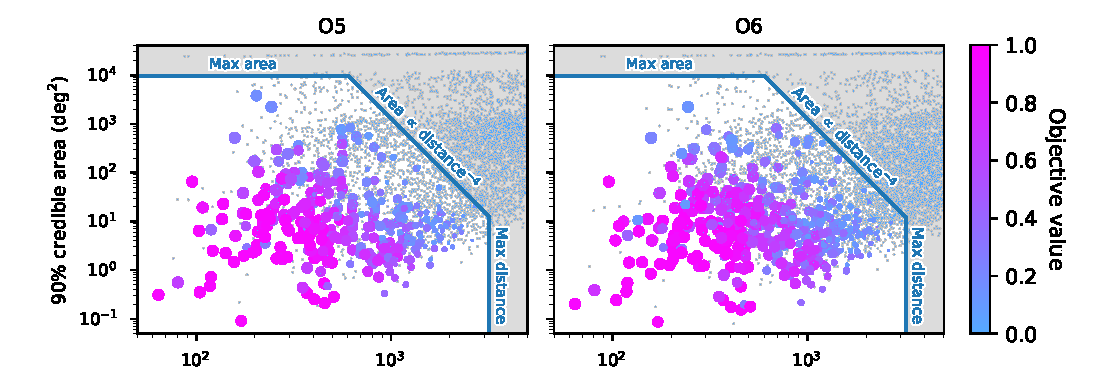
\includegraphics[width=\textwidth]{figures/area-distance}
    \caption{\label{fig:area-distance}90\% credible area and distance of simulated \ac{GW} events. Events that were selected for follow-up with \ac{UVEX} are represented by colored dots, with the color of the dot representing the scheduler objective value and the area of the dot the detection probability. Events that were not selected for follow-up are marked with gray dots. The blue boundary represents the analytical predictor of the detection threshold given by Eqs.~(\ref{eq:threshold-distance},\ref{eq:threshold-area},\ref{eq:threshold-area-distance}).}
\end{figure*}

\begin{deluxetable}{lcc}
    \tablecaption{\label{tab:selected-detected}Expected number of events selected for follow-up and detected.}
    \tablehead{& O5 & O6}
    \startdata
    Number of events selected & $51_{-31}^{+67}$ & $72_{-42}^{+93}$ \\
Number of events detected & $26_{-16}^{+35}$ & $38_{-23}^{+51}$

    \enddata
\end{deluxetable}

\subsection{Comparison with greedy method}

\section{Conclusion}

\begin{acknowledgments}
This work was performed in part at the Aspen Center for Physics, which is supported by \ac{NSF} grant PHY-2210452.

This work used Expanse at \ac{SDSC} through allocation AST200029, ``Towards a complete catalog of variable sources to support efficient searches for compact binary mergers and their products,'' from the Advanced Cyberinfrastructure Coordination Ecosystem: Services \& Support (ACCESS) program, which is supported by \ac{NSF} grants \#2138259, \#2138286, \#2138307, \#2137603, and \#2138296.
\end{acknowledgments}

\vspace{5mm}
\software{
    astropy \citep{2013A&A...558A..33A,2018AJ....156..123A},
    dust\_extinction \citep{2024JOSS....9.7023G},
    dustmaps \citep{2018JOSS....3..695M},
    HEALPix \citep{2005ApJ...622..759G},
    healpy \citep{2019JOSS....4.1298Z},
    ligo.skymap \citep{2016PhRvD..93b4013S,2016ApJ...829L..15S,2016ApJS..226...10S},
    synphot \citep{2018ascl.soft11001S}}

\bibliography{m4opt}{}
\bibliographystyle{aasjournal}

\end{document}
